\documentclass[tikz, border=5pt]{standalone}
\usepackage{tikz}

\begin{document}
	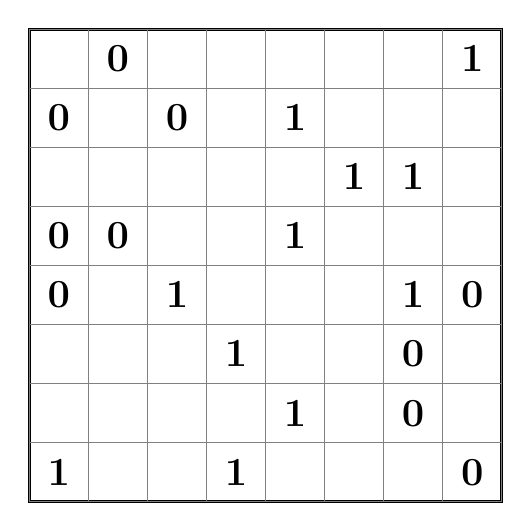
\begin{tikzpicture}[scale=0.75]
		% Dibujo de la cuadrícula
		\draw[very thick] (0,0) rectangle (8,8);
		\draw[step=1cm, gray, thin] (0,0) grid (8,8);
		
		% Matriz inicial del tablero
		% Fila 1 (y=7)
		\node at (1.5, 7.5) {\Large\bfseries 0};
		\node at (7.5, 7.5) {\Large\bfseries 1};
		
		% Fila 2 (y=6)
		\node at (0.5, 6.5) {\Large\bfseries 0};
		\node at (2.5, 6.5) {\Large\bfseries 0};
		\node at (4.5, 6.5) {\Large\bfseries 1};
		
		% Fila 3 (y=5)
		\node at (5.5, 5.5) {\Large\bfseries 1};
		\node at (6.5, 5.5) {\Large\bfseries 1};
		
		% Fila 4 (y=4)
		\node at (0.5, 4.5) {\Large\bfseries 0};
		\node at (1.5, 4.5) {\Large\bfseries 0};
		\node at (4.5, 4.5) {\Large\bfseries 1};
		
		% Fila 5 (y=3)
		\node at (0.5, 3.5) {\Large\bfseries 0};
		\node at (2.5, 3.5) {\Large\bfseries 1};
		\node at (6.5, 3.5) {\Large\bfseries 1};
		\node at (7.5, 3.5) {\Large\bfseries 0};
		
		% Fila 6 (y=2)
		\node at (3.5, 2.5) {\Large\bfseries 1};
		\node at (6.5, 2.5) {\Large\bfseries 0};
		
		% Fila 7 (y=1)
		\node at (4.5, 1.5) {\Large\bfseries 1};
		\node at (6.5, 1.5) {\Large\bfseries 0};
		
		% Fila 8 (y=0)
		\node at (0.5, 0.5) {\Large\bfseries 1};
		\node at (3.5, 0.5) {\Large\bfseries 1};
		\node at (7.5, 0.5) {\Large\bfseries 0};
	\end{tikzpicture}
\end{document}